\section{Zielsetzung}
Ziel dieses Versuchs ist die Bestimmung einzelner Bauteile im elektrischen Schaltkreis,
sowie die Ermittlung der Frequenzabhängigkeit der Brückenspannung einer Wien-Robinson-Brücke.

\section{Theorie}
    \label{sec:Theorie}
    Die Inhalte des Theorieteils sind auf Grundlage des Dokuments \cite{V302_Anleitung} zusammengetragen.
    Brückenschaltungen sind eine essenzielle Messmethode, da sie sehr viel präziser sind als herkömmliche Methoden.
    Besondere Bedeutung bekommt dabei die Nullmethode, welche die zu messende Größe mit einer hohen Genauigkeit bestimmt.
    Hierbei wird die sogenannte Brückenspannung abgeglichen.
    Dabei ist es wichtig, dass sich jede physikalische Größe durch Widerstände ausdrücken lässt.
    \subsection{Allgemeine Brückenschaltung}
    Bei der allgemienen Brückenschaltung sind alle Widerstände bekannt und die Brückenspannung zwischen A und B (siehe
    Abb. \ref{fig:All_Brueckenschaltung}) kann berechnet werden.
    \begin{figure}
        \centering
        \includegraphics[height=5cm]{Allgemeine_Brückenschaltung.jpg}
        \caption{Prinzipielle Brückenschaltung}
        \label{fig:All_Brueckenschaltung}
    \end{figure}
    Dafür werden die zwei Kirchhoffschen Gesetzte verwendet.
    \begin{enumerate}
        \item Die Maschenregel besagt, dass in jedem in sich geschlossenen Stromkreis die Summe der Spannung gleich null ist.
    \end{enumerate}
    Aufgrund der Kontenregel gilt $I_1 = I_2$ und $I_3 = I_4$.
    Mit der Maschenregel ergibt sich $U = -R_1 I_1 + R_3 I_3$ und $U = R_2 I_2 - R_4 I_4$.
    Außerdem ist die Speisespannung der Brücke gegeben durch $U_\text{S} = I_1(R_1 + R_2)$.
    So berechnet sich die Spannung U zwischen A und B mit
    \begin{equation}
        U = \frac{R_2 R_3 - R_1 R_4}{(R_3 + R_4)(R_1 + R_2)}U_{\text{S}} \, \text{.}
        \label{eq:Brueckenspannung}
    \end{equation}
    Hierbei gelten die Bezeichnungen gemäß Abb. \ref{fig:All_Brueckenschaltung}.
    \subsection{Abgeglichene Brücke}
    Als abgeglichene Brücke wird der Fall bezeichnet, bei dem die Brückenspannung gleich null ist.
    Dies ist dann erreicht, wenn
    \begin{equation}
        R_1 R_4 = R_2 R_3
        \label{eq:Abgleichbed}
    \end{equation}
    ist.
    Durch diese Abgleichbedingung kann eine Widerstandsmessung durchgeführt werden, da die Brückenspannung
    nur von dem Verhältnis der Widerstände abhängt.
    Wie Gl. \eqref{eq:Brueckenspannung} zeigt, ist $U$ proportional zu $U_{\text{S}}$.
    Also muss $U_{\text{S}}$ möglichst groß gewählt werden, damit die Genauigkeit der Messung verbessert wird.
    \subsection{Wheatstonsche Brücke}
    Die Wheastosche Brücke wird zur Bestimmung unbekannter Widerstände genutzt.
    Diese Brücke ist aufgebaut gemäß Abb. \ref{fig:Wheastonsche_Bruecke}.
    \begin{figure}
        \centering
        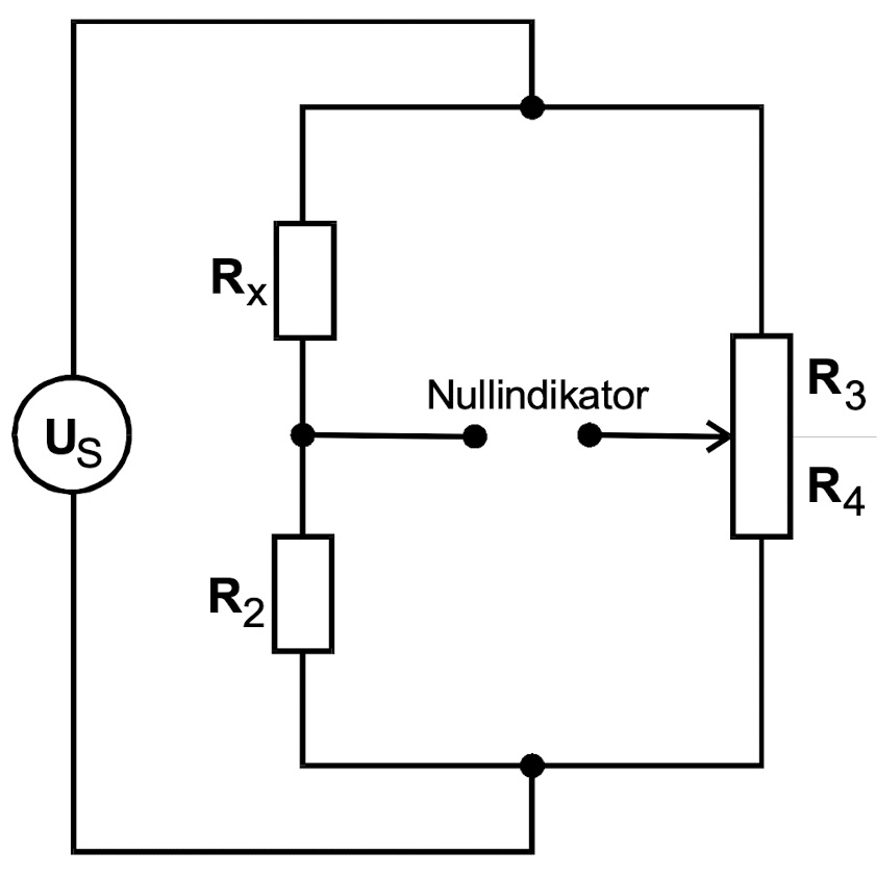
\includegraphics[height= 5cm]{Messdaten/Wheastonsche-Brueke.jpg}
        \caption{Wheastonsche Brückenschaltung}
        \label{fig:Wheastonsche_Bruecke}
    \end{figure}
    Um den unbekannten Widerstand $R_x$ zu bestimmen, wird die Abgleichbedingung \eqref{eq:Abgleichbed} nach $R_x$ umgestellt.
    Somit ergibt sich
    \begin{equation*}
        R_x = R_2 \frac{R_3}{R_4} \, \text{.}
    \end{equation*}
    \subsection{Kapazitätsmessbrücke}
    Auch komplexe Widerstände können mit diesem Prinzip ermittelt werden.
    Ein solches Schaltbild ist in Abb. \ref{fig:Kapatitaetsmessbruecke} dargestellt.
    \begin{figure}
        \centering
        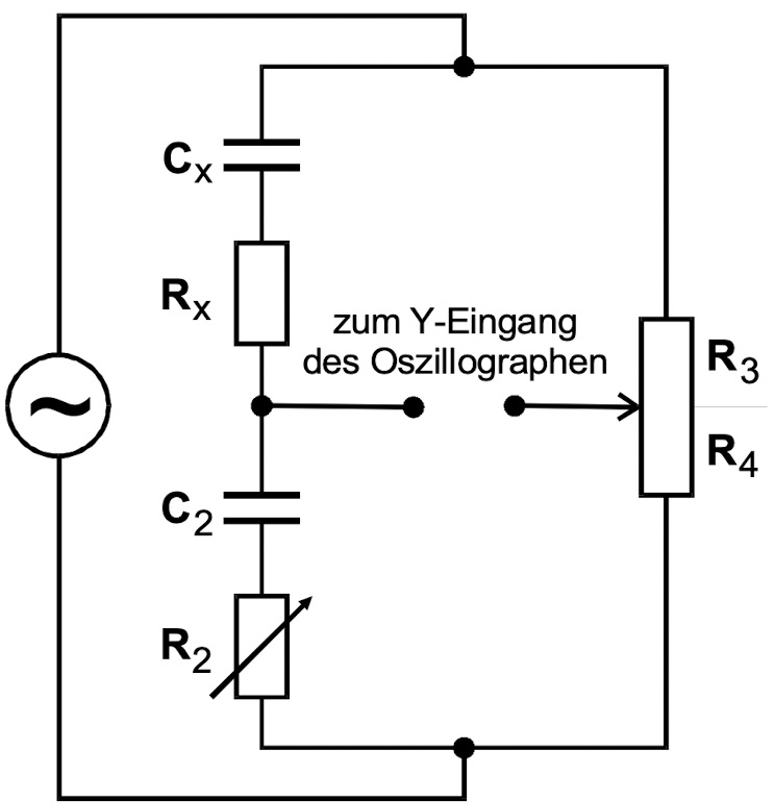
\includegraphics[height= 5cm]{Messdaten/Kapazitaetsmessung.jpg}
        \caption{Kapazitätsmessbrücke für Kondensatoren mit dielektischen Verlusten}
        \label{fig:Kapatitaetsmessbruecke}
    \end{figure}
    Um die Verlustleistung des zu ermittlenden Kondensator mit zu berücksichtigen, wird ein Widerstand mit diesem in Reihe geschaltet
    und das typische Ersatzschaltbild eines realen Kondensators, entsteht.
    $R_x$ wird wieder über die Abgleichbedingung \eqref{eq:Abgleichbed} bestimmt.
    $C_x$ ergibt sich zu
    \begin{equation}
         C_x = C_2 \frac{R_4}{R_3} \, \text{.}
         \label{eq:kapawiderstand}
    \end{equation}
    \subsection{Induktivitätsmessbrücke}
    Zur Bestimmung der Induktivität einer Spule gelten gleich Bedingungen wie bei der Kapazitasmessung.
    \begin{figure}
        \centering
        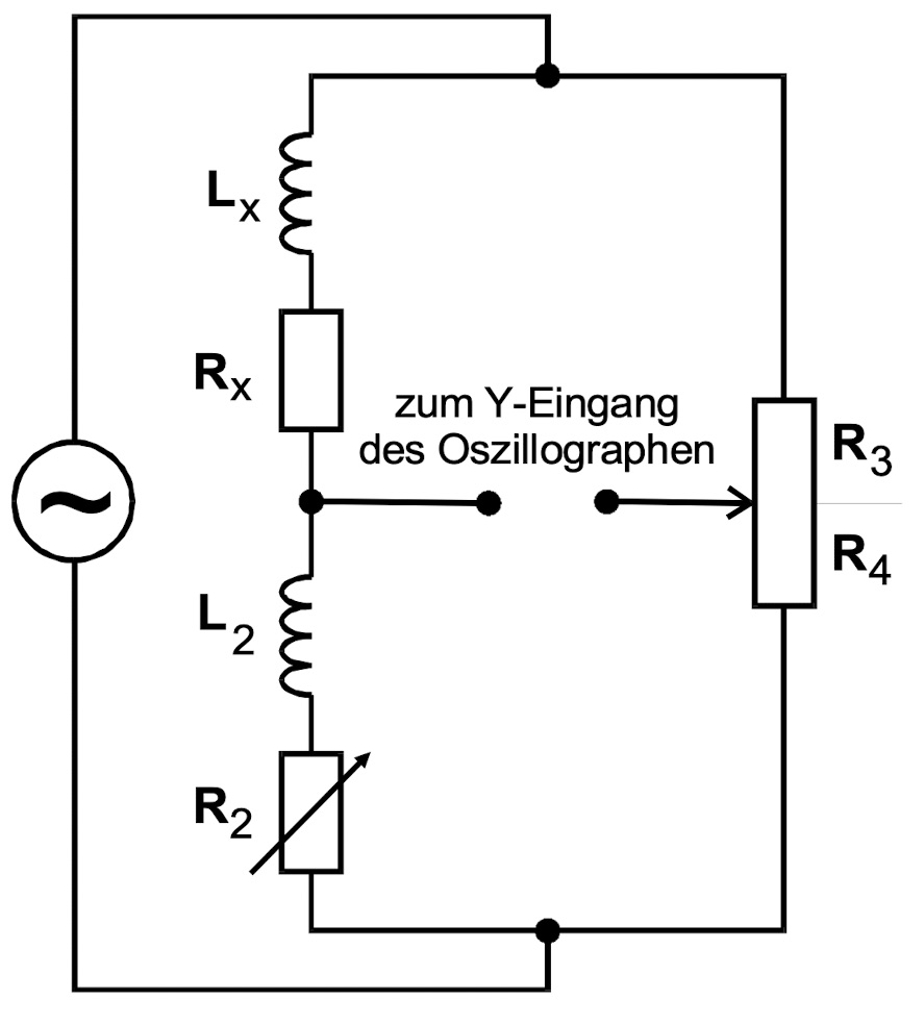
\includegraphics[height=5cm]{Induktivitaetsmessung.jpg}
        \caption{Messbrücke für verlustbehaftete Induktivitäten}
        \label{fig:Induktivitaetsmessbruecke}
    \end{figure}
    Somit ist das Schaltbild, wie in Abb. \ref{fig:Induktivitaetsmessbruecke} dargestellet.
    $R_x$ wird wieder über die Abgleichbedingung \eqref{eq:Abgleichbed} berechnet.
    Für $L_x$ ergibt sich
    \begin{equation}
        L_x = L_2 \frac{R_3}{R_4}\, \text{.}
        \label{eq:induktivität}
    \end{equation}
    \subsection{Maxwell-Brücke}
    Die Maxwell-Brücke (sieht Abb. \ref{fig:Maxwell_Bruecke}) ist eine andere Brücke zur Untersuchung der Induktivität einer Spule.
    \begin{figure}
        \centering
        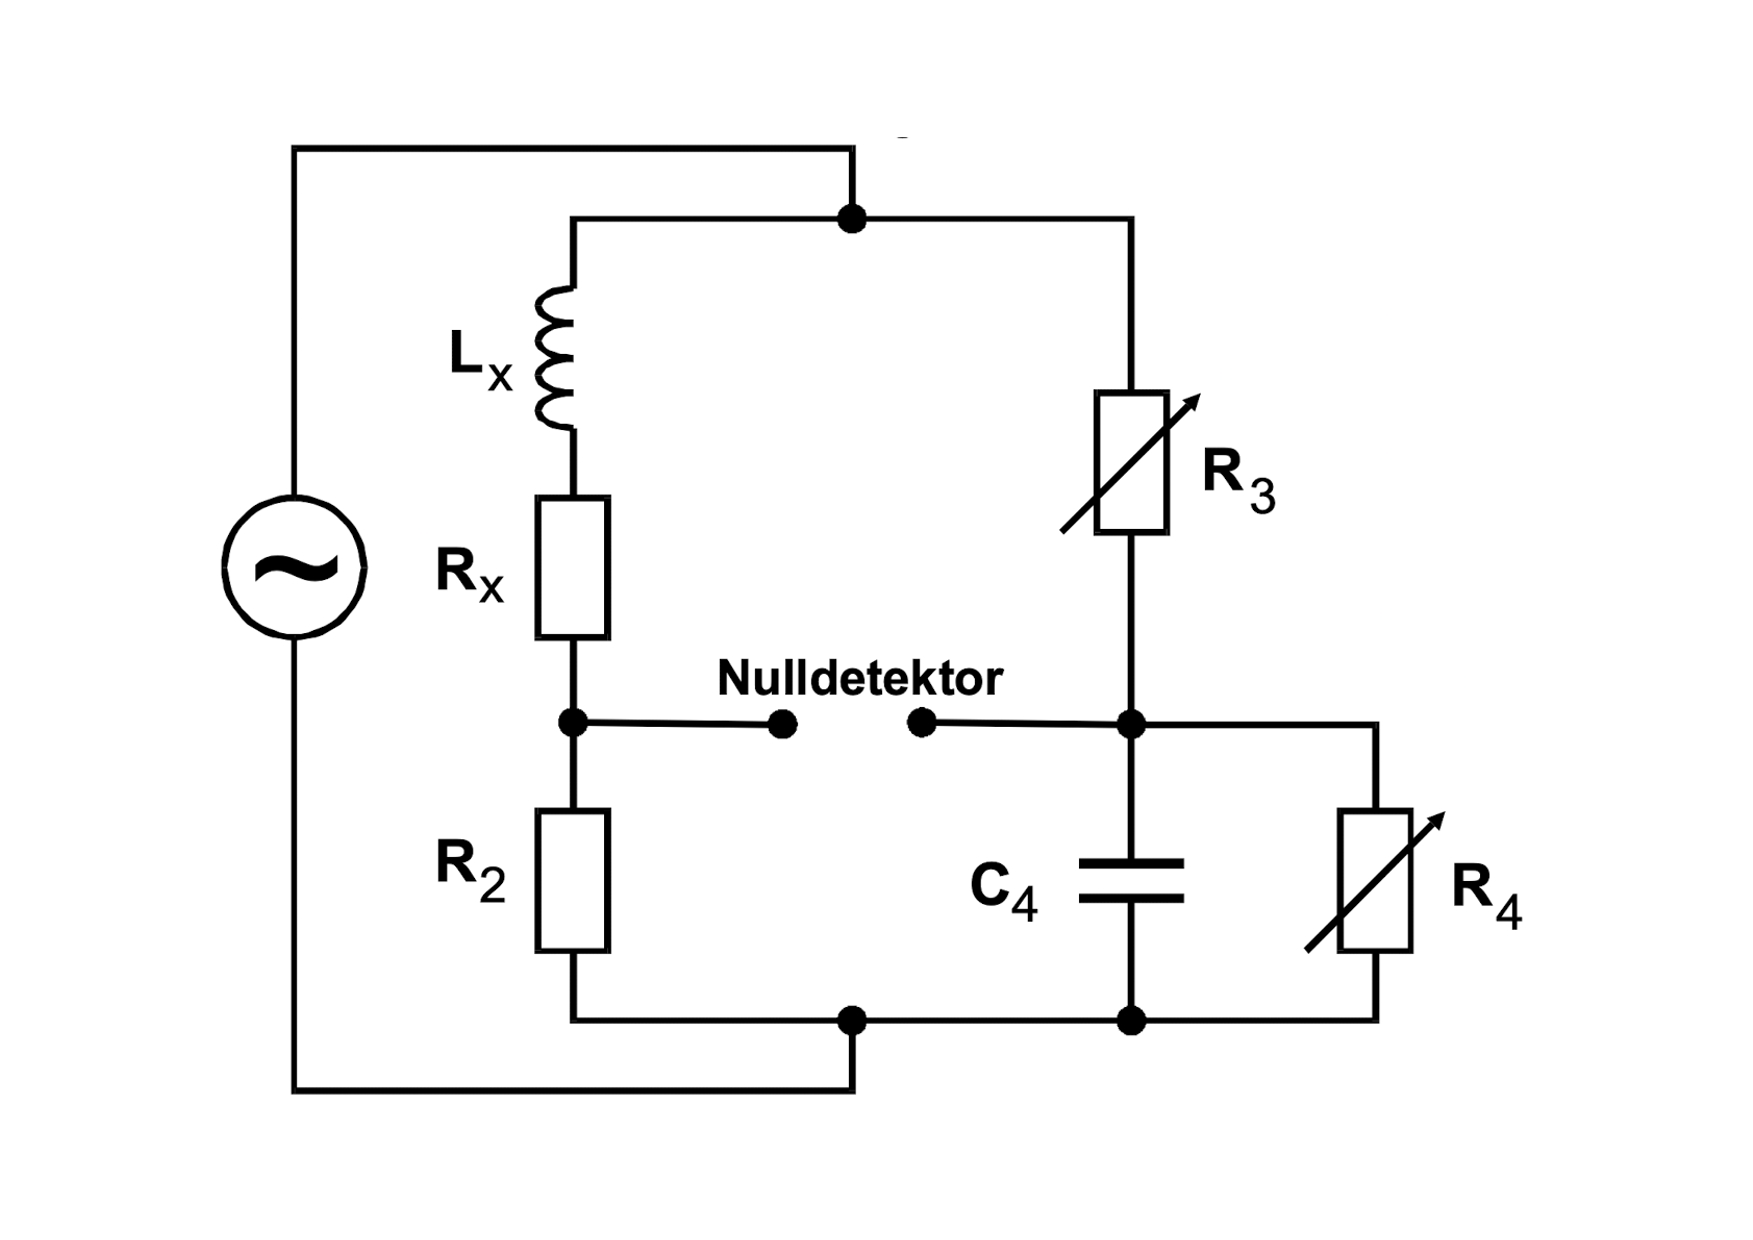
\includegraphics[height= 5cm]{Messdaten/Maxwell.jpg}
        \caption{Maxwell-Brücke zur Messung einer verlustbehafteten Induktivität}
        \label{fig:Maxwell_Bruecke}
    \end{figure}
    Mit den Kirchhoffschen Gesetzen lassen sich wieder Gesetzmäßigkeiten für die Verhältnisse der Widerstände aufstellen.
    So wird $R_x$ über die Abgleichbedingung \eqref{eq:Abgleichbed} und $L_x$ mit
    \begin{equation}
        L_x = R_2 R_3 C_4
        \label{eq:maxwell}
    \end{equation}
    bestimmt.
    \subsection{Wien-Robinson-Brücke}
    Bei der Wien-Robinson-Brücke, in Abb. \ref{fig:Wien_Robinson_Bruecke} dargestellt, sind keine Abgleichelemente mehr enthalten.
    Der Abgleich erfolgt hier über die veränderbare Frequenz der Speisespannung $U_\text{S}$.
    \begin{figure}
        \centering
        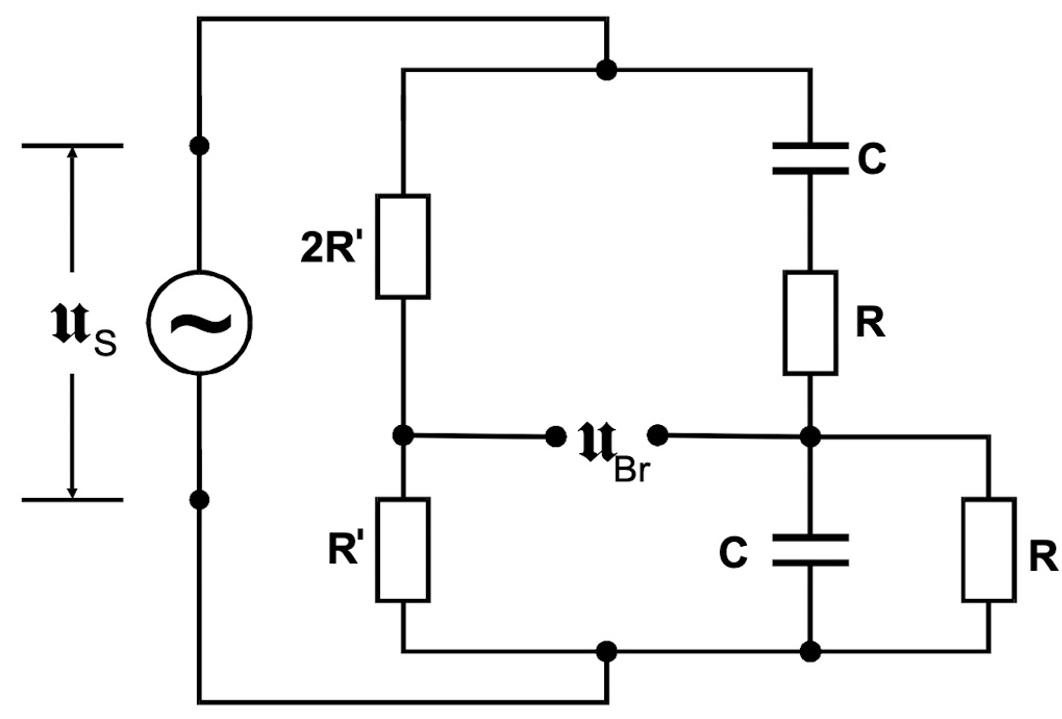
\includegraphics[height=5cm]{Messdaten/Wien-Robinson-Bruecke.jpg}
        \caption{Schaltbild einer Wien-Robinson-Brücke.}
        \label{fig:Wien_Robinson_Bruecke}
    \end{figure}
    Durch Überlegungen mit den Kirchhoffschen Gesetzen, kann erkannt werden, dass die Brückenspannung genau dann verschwindet,
    wenn $\omega_0 = \sfrac{1}{RC}$ gilt.
    Wobei $\omega_0$ die Frequenz ist, bei der die Brückenspannung minimal wird.
    Anschließend wird das Verhältnis von $\omega_0$ zu $\omega$ eingeführt
    \begin{equation*}
        \Omega = \frac{\omega}{\omega_0}\, \text{.}
    \end{equation*}
    Damit ergibt sich das Betragsquadrat des Verhältnisses zwischen Speise- und Brückenspannung
    \begin{equation}
        |\frac{U_\text{Br}}{U_\text{S}}|^2 = \frac{1}{9} \frac{(\Omega^2 - 1)^2}{(1 - \Omega^2)^2 + 9 \Omega^2} \, \text{.}
    \label{eq:theoriekurve}
    \end{equation}
    Der Klirrfaktor $k$ wird mittels
    \begin{equation}
        k = \frac{\sqrt {U_2^2 + U_3^2 + \dotsb}}{U_1}
    \end{equation}
    bestimmt.
    Hierbei ist $U_1$ die Amplitude der Grundwelle und $U_\text{n}$ die Amplitude der n-ten Oberwelle mit der Frequenz $n\omega_0$.
    Um dies zu vereinfachen, wird nur die Spannung der ersten Oberwelle $U_2$ betrachtet.
    So ergibt sich
    \begin{equation}
        k = \frac{U_2}{U_1} \, \text{.}
    \end{equation}
    Für die Spannung $U_2$ gilt
    \begin{equation}
        U_2 = \frac{U_\text{Br}}{f(\Omega = 2)} \, \text{.}
    \end{equation}
    Damit lässt sich der Klirrfaktor $k$ berechnen.